% This is text associated with the open textbook "Open Electromagnetics"
% See immediately below for author, date
% This work is licensed under the Creative Commons Attribution-ShareAlike 4.0 International License. (CC BY-SA 4.0) 
% To view a copy of the license, visit http://creativecommons.org/licenses/by-sa/4.0/

%ORB TITLE Far-Field Radiation from a Thin Straight Filament of Current
%ORB AUTHOR 0        # S.W. Ellingson, Virginia Tech (ellingson@vt.edu)
%ORB DATE 20191128   # yyyymmdd
%ORB ABSTRACT 

\label{m0199_Radiation_from_a_Thin_Straight_Filament_of_Current} % <-- Must match name of this file and module directory name.  Don't mess with this!

A simple distribution of radiating current that is encountered in common practice is the thin straight current filament, shown in Figure~\ref{m0199_fTSCF}.
%
\begin{figure}[b!] % <--- "[b!]" for first figure in section *only*; delete for 2nd and subsequent figures
\begin{center}
\pdftooltip{{  % note double braces
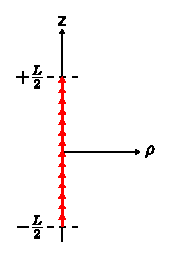
\includegraphics[width=1.5in]{modules/m0199_fCF.eps} 
% https://commons.wikimedia.org/wiki/File:A_thin_straight_distribution_of_radiating_current.svg
}}{A rho-z coordinate system. A series of red arrows point up along the z axis from negative capital L over 2 to positive capital L over 2.}
\end{center}
\centerline{\scriptsize 
\copyright~\hyperref[m0199_fTSCF_Credit]{C.\ Wang} 
\href{https://creativecommons.org/licenses/by-sa/4.0/}{CC BY-SA 4.0} 
} % \centerline 
\caption{
\label{m0199_fTSCF}
A thin straight distribution of radiating current.
}
\end{figure}
%
The defining characteristic of this distribution is that the current filament is aligned along a straight line, and that the maximum dimension of the cross-section of the filament is much less than a wavelength.
The latter characteristic is what we mean by ``thin'' -- i.e., the filament is ``electrically thin.''
Physical distributions of current that meet this description include the electrically-short dipole 
\index{antenna!electrically-short dipole (ESD)}
(Section~\ref{m0198_Radiation_from_an_Electrically-Short_Dipole})
 and the half-wave dipole 
\index{antenna!half-wave dipole}
(Section~\ref{m0200_Radiation_from_a_Half-Wave_Dipole})
among others.
A gentler introduction to this distribution is via Section~\ref{m0198_Radiation_from_an_Electrically-Short_Dipole} (``Radiation from an Electrically-Short Dipole''), so students may want to review that section first.  This section presents the more general case.

Let the magnitude and phase of current along the filament be given by the phasor quantity $\widetilde{I}(z)$ (SI base units of A).
In principle, the only constraint on $\widetilde{I}(z)$ that applies generally is that it must be zero at the ends of the distribution; i.e., $\widetilde{I}(z) = 0$ for $\left|z\right|\ge L/2$.
Details beyond this constraint depend on $L$ and perhaps other factors.
Nevertheless, the characteristics of radiation from members of this class of current distributions have much in common, regardless of $L$.
These become especially apparent if we limit our scope to field points far from the current, as we shall do here.

There are two approaches that we might consider in order to find the electric field radiated by this distribution.
The first approach is to calculate the magnetic vector potential 
\index{magnetic vector potential}
$\widetilde{\bf A}$ by integration over the current distribution (Section~\ref{m0196_Solution_of_the_Wave_Equation_for_Magnetic_Vector_Potential}), 
calculate $\widetilde{\bf H}=(1/\mu)\nabla\times\widetilde{\bf A}$, and finally calculate $\widetilde{\bf E}$ from $\widetilde{\bf H}$ using the differential form of Ampere's law.
\index{Ampere's law!general form}
In this section, we shall employ a simpler approach, shown in Figure~\ref{m0199_fCFHD}.
%
\begin{figure} % <--- "[b!]" for first figure in section *only*; delete for 2nd and subsequent figures
\begin{center}
\pdftooltip{{  % note double braces
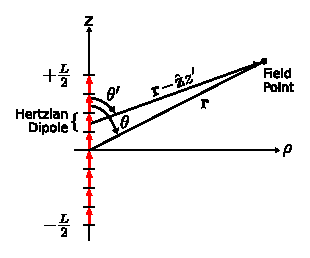
\includegraphics[width=2.5in]{modules/m0199_fCFHD.eps} 
% https://commons.wikimedia.org/wiki/File:Esd_approximated_as_a_large_number_of_hertzian_dipoles.svg
}}{A rho-z coordinate system. Small arrows run the length of the z axis from a distance negative capital L over 2 to positive capital L over 2. A single arrow is labeled Hertzian Dipole. Vector small r goes from the origin to field point in rho-z axis at an angle theta from the positive z axis. A second vector originates 1.5 arrows lengths to the field point forms an angle theta prime with the z axis. Its length is boldface small r minus boldface z hat times z. The angle vector small r makes with the z axis is theta.}
\end{center}
\centerline{\scriptsize 
\copyright~\hyperref[m0199_fCFHD_Credit]{C.\ Wang} 
\href{https://creativecommons.org/licenses/by-sa/4.0/}{CC BY-SA 4.0} 
} % \centerline 
\caption{
\label{m0199_fCFHD}
Current distribution approximated as a set of Hertzian dipoles.
}
\end{figure}
%
Imagine the filament as a collection of many shorter segments of current that radiate independently.
The total field is then the sum of these short segments.
Because these segments are very short relative to the length of the filament as well as being short relative to a wavelength, we may approximate the current over each segment as constant. 
In other words, we may interpret each segment as being, to a good approximation, a Hertzian dipole.
\index{Hertzian dipole}

The advantage of this approach is that we already have a solution for every segment.
In Section~\ref{m0197_Radiation_from_a_Hertzian_Dipole}, it is shown that a $\hat{\bf z}$-directed Hertzian dipole at the origin radiates the electric field
%
\begin{equation}
\widetilde{\bf E}({\bf r}) \approx \hat{\bf \theta} j\eta \frac{\widetilde{I}\left(\beta \Delta l\right)}{4\pi}~\left(\sin\theta\right) \frac{e^{-j\beta r}}{r} 
\end{equation}
%
where $\widetilde{I}$ and $\Delta l$ may be interpreted as the current and length of the filament, respectively.
In this expression, $\eta$ is the wave impedance of medium in which the filament radiates (e.g., $\approx 377~\Omega$ for free space), and we have presumed lossless media such that the attenuation constant $\alpha\approx 0$ and the phase propagation constant $\beta=2\pi/\lambda$.   
This expression also assumes field points far from the filament; specifically, distances $r$ that are much greater than $\lambda$.
Repurposing this expression for the present problem, we note that the segment at the origin radiates the electric field:
%
\begin{equation}
\widetilde{\bf E}({\bf r};z'=0) \approx \hat{\bf \theta} j\eta \frac{\widetilde{I}(0)\left(\beta \Delta l\right)}{4\pi}~\left(\sin\theta\right) \frac{e^{-j\beta r}}{r} 
\end{equation}
%
where the notation $z'=0$ indicates the Hertzian dipole is located at the origin.
Letting the length $\Delta l$ of this segment shrink to differential length $dz'$, we may describe the contribution of this segment to the field radiated by the ESD as follows:
%
\begin{equation}
d\widetilde{\bf E}({\bf r};z'=0) \approx \hat{\bf \theta} j\eta \frac{\widetilde{I}(0)\left(\beta dz'\right)}{4\pi}~\left(\sin\theta\right) \frac{e^{-j\beta r}}{r} 
\end{equation}
% 
Using this approach, the electric field radiated by \emph{any} segment can be written:
%
\begin{equation}
d\widetilde{\bf E}({\bf r};z') \approx 
\hat{\bf \theta}' j\eta\beta \frac{\widetilde{I}(z')}{4\pi}\left(\sin\theta'\right) \frac{e^{-j\beta \left|{\bf r}-\hat{\bf z}z'\right|}}{\left|{\bf r}-\hat{\bf z}z'\right|}~dz'
\end{equation}
%
Note that $\theta$ is replaced by $\theta'$ since the ray ${\bf r}-\hat{\bf z}z'$ forms a different angle (i.e., $\theta'$) with respect to $\hat{\bf z}$.
Subsequently, $\hat{\bf \theta}$ is replaced by $\hat{\bf \theta}'$, which varies similarly with $z'$.
The electric field radiated by the filament is obtained by integration over these contributions, yielding:
%
\begin{equation}
\widetilde{\bf E}({\bf r}) \approx \int_{-L/2}^{+L/2} d\widetilde{\bf E}(\hat{\bf r};z') 
\end{equation}
%
Expanding this expression:
%
\begin{equation}
\widetilde{\bf E}({\bf r}) \approx 
 j \frac{\eta\beta}{4\pi} \int_{-L/2}^{+L/2} \hat{\bf \theta}' \widetilde{I}(z')~\left(\sin\theta'\right) \frac{e^{-j\beta \left|{\bf r}-\hat{\bf z}z'\right|}}{\left|{\bf r}-\hat{\bf z}z'\right|} dz'
\end{equation}
%
Given some of the assumptions we have already made, this expression can be further simplified.
For example, note that $\theta'\approx\theta$ since $L\ll r$.
For the same reason, $\hat{\bf \theta}'\approx\hat{\bf \theta}$.
Since these variables are approximately constant over the length of the filament, we may move them outside the integral, yielding:
%
\begin{equation}
\widetilde{\bf E}({\bf r}) \approx \hat{\bf \theta} j \frac{\eta\beta}{4\pi}~\left(\sin\theta\right) \int_{-L/2}^{+L/2} \widetilde{I}(z') \frac{e^{-j\beta \left|{\bf r}-\hat{\bf z}z'\right|}}{\left|{\bf r}-\hat{\bf z}z'\right|} dz'
\label{m0199_eE1}
\end{equation}

It is also possible to simplify the expression $\left|{\bf r}-\hat{\bf z}z'\right|$.
Consider Figure~\ref{m0199_fParallelRays}.
%
\begin{figure} % <--- "[b!]" for first figure in section *only*; delete for 2nd and subsequent figures
\begin{center}
\pdftooltip{{  % note double braces
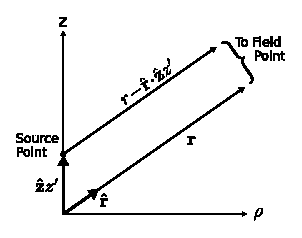
\includegraphics[width=2.5in]{modules/m0199_fParallelRays.eps} 
% https://commons.wikimedia.org/wiki/File:Parallel_ray_approximation_for_an_esd.svg
}}{A rho-z coordinate system. Vector small r starts at the origin and points towards a field point in the positive z and positive rho direction. A short vector boldface small r hat overlays the small r vector. A third vector originates at the origin and goes in the positive z direction to a source point. It is a length boldface small z hat times z prime. A fourth vector originates at the source point and stretches towards the field point. It runs parallel to the small r vector.}
\end{center}
\centerline{\scriptsize 
\copyright~\hyperref[m0199_fParallelRays_Credit]{C.\ Wang} 
\href{https://creativecommons.org/licenses/by-sa/4.0/}{CC BY-SA 4.0} 
} % \centerline 
\caption{
\label{m0199_fParallelRays}
Parallel ray approximation.
}
\end{figure}
%
Since we have already assumed that $r\gg L$ (i.e., the distance to field points is much greater than the length of the filament), the vector ${\bf r}$ is approximately parallel to the vector ${\bf r}-\hat{\bf z}z'$.
Subsequently, it must be true that
%
\begin{flalign}
\left|{\bf r}-\hat{\bf z}z'\right| &\approx r-\hat{\bf r}\cdot\hat{\bf z}z' \label{m0199_ePRA} \\
                                   &\approx r-z'\cos{\theta} 
\end{flalign}
%
Note that the magnitude of $r-\hat{\bf r}\cdot\hat{\bf z}z'$ must be approximately equal to $r$, since $r\gg L$.
So, insofar as $\left|{\bf r}-\hat{\bf z}z'\right|$ determines the \emph{magnitude} of $\widetilde{\bf E}({\bf r})$, we may use the approximation:
%
\begin{equation}
\left|{\bf r}-\hat{\bf z}z'\right| \approx r ~~~\mbox{(magnitude)}
\end{equation}
%
Insofar as $\left|{\bf r}-\hat{\bf z}z'\right|$ determines \emph{phase}, we have to be more careful.
The part of the integrand of Equation~\ref{m0199_eE1} that exhibits varying phase is $e^{-j\beta \left|{\bf r}-\hat{\bf z}z'\right|}$.
Using Equation~\ref{m0199_ePRA}, we find
%
\begin{equation}
e^{-j\beta\left|{\bf r}-\hat{\bf z}z'\right|} \approx e^{-j\beta r} e^{+j\beta z'\cos{\theta}}
\end{equation}
%
These simplifications are known collectively as a \emph{far field approximation}, 
\index{far field}
since they are valid only for distances ``far'' from the source.

Applying these simplifications for magnitude and phase to Equation~\ref{m0199_eE1}, we obtain:
%
\begin{flalign}
\widetilde{\bf E}({\bf r}) &\approx \hat{\bf \theta} j \frac{\eta\beta}{4\pi} \frac{e^{-j\beta r}}{r}~\left(\sin\theta\right) \nonumber \\
                           & ~~~\cdot\int_{-L/2}^{+L/2} \widetilde{I}(z') e^{+j\beta z'\cos{\theta}} dz'
\end{flalign}
%
Finally, it is common to eliminate the factor of $\beta$ in the magnitude using the relationship $\beta=2\pi/\lambda$, yielding:
%
\begin{flalign}
%\boxed{
\widetilde{\bf E}({\bf r}) &\approx \hat{\bf \theta} j \frac{\eta}{2} \frac{e^{-j\beta r}}{r}~\left(\sin\theta\right) \nonumber \\
                           & ~~~\cdot\left[\frac{1}{\lambda}\int_{-L/2}^{+L/2} \widetilde{I}(z') e^{+j\beta z'\cos{\theta}} dz'\right] \label{m0199_eESDE}
%}
\end{flalign}
%
%%%%%%%%%%%%%%%%%%%%%%%%%%%%%%%%%%%%%%%%%%%%%%%
%ORB HIGHLIGHT
\begin{mdframed}[backgroundcolor=yellow!20,nobreak=true] 
The electric field radiated by a thin, straight, $\hat{\bf z}$-directed current filament of length $L$ located at the origin and aligned along the $z$ axis is given by Equation~\ref{m0199_eESDE}.
This expression is valid for $r\gg L$ and $r\gg\lambda$.
\end{mdframed}
%%%%%%%%%%%%%%%%%%%%%%%%%%%%%%%%%%%%%%%%%%%%%%%

At field points satisfying the conditions $r\gg L$ and $r\gg\lambda$, the wave appears to be locally planar.
Therefore, we are justified using the plane wave relationship
\index{plane wave relationships}
$ \widetilde{\bf H} = (1/\eta) \hat{\bf r} \times \widetilde{\bf E} $
to calculate $\widetilde{\bf H}$.

As a check, one may readily verify that Equation~\ref{m0199_eESDE} yields the expected result for the electrically-short dipole 
\index{antenna!electrically-short dipole (ESD)}
(Section~\ref{m0198_Radiation_from_an_Electrically-Short_Dipole}).  

